\documentclass{article}
\usepackage{amsmath, sfmath, multicol, tkz-euclide, array, enumerate, tcolorbox, tabularray, tipa}
\renewcommand{\familydefault}{\sfdefault}
\setlength{\parindent}{0cm}
\pagestyle{empty}
\usepackage[left=1in, top=0.5in, right=1in, bottom=0.5in]{geometry}
\tikzset{>=stealth, label style/.append style={font=\footnotesize}}
\tcbset{colback=white}

\newcounter{example}[section]
\newenvironment{example}[1][]{\refstepcounter{example}\par\medskip
   {\color{red}\textbf{Example~\theexample. #1}}}{\medskip}

\newcommand{\arc}[1]{%
    \setbox9=\hbox{#1}%
    \ooalign{\resizebox{\wd9}{\height}{\texttoptiebar{\phantom{A}}}\cr#1}}

\begin{document}

\section*{Nets and Drawings}

\begin{tcolorbox}[colframe=orange!70!white, coltitle=black, title=\textbf{Today I Can}]
\begin{enumerate}
    \item Make nets and drawings of 3-dimensional figures.
\end{enumerate}
\end{tcolorbox}
\smallskip 

\begin{tcolorbox}[colframe=black!20!white, opacitybacktitle=0.1, coltitle=black, title=\textbf{Net}]
A 2-D diagram that you can form into a 3-D figure. A net shows all of the surfaces of a figure in one view.
\end{tcolorbox}
\smallskip 

\begin{example}
The net below folds into a cube.
\begin{enumerate}[(a)]
    \item Which letters will be on the top and front of the cube?   \newline\\

    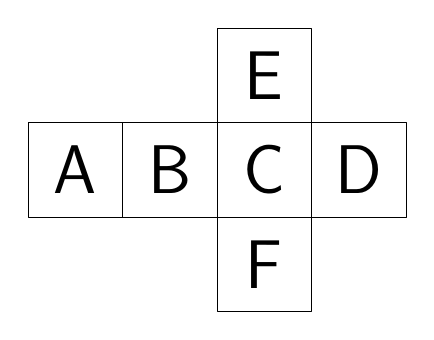
\begin{tikzpicture}[scale=0.6]
    \tkzDefPoints{0/0/A, 2/0/B, 4/0/C, 6/0/D, 8/0/E, 8/2/F, 6/2/G, 4/2/H, 2/2/I, 0/2/J, 4/-2/K, 6/-2/L, 4/4/M, 6/4/N}
    \tkzDrawPolygon(A,E,F,J)
    \tkzDrawPolygon(C,K,L,D)
    \tkzDrawPolygon(H,G,N,M)
    \tkzDrawSegments(B,I C,H D,G)
    \node at (1,1) {\Huge A};
    \node at (3,1) {\Huge B};
    \node at (5,1) {\Huge C};
    \node at (7,1) {\Huge D};
    \node at (5,3) {\Huge E};
    \node at (5,-1) {\Huge F};
    \end{tikzpicture}
    \hspace{1in}
    \raisebox{1cm}
    {
    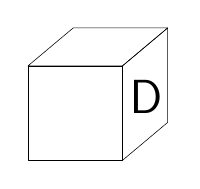
\begin{tikzpicture}[scale=0.6]
    \tkzDefPoints{0/0/A, 2/0/B, 2/2/C, 0/2/D}
    \tkzDrawPolygon(A,B,C,D)
    \tkzDefShiftPoint[D](40:1.25){E}
    \tkzDefShiftPoint[C](40:1.25){F}
    \tkzDrawPolygon(D,C,F,E)
    \tkzDefShiftPoint[B](40:1.25){G}
    \tkzDrawPolygon(B,G,F,C)
    \node at (2.5,1.35) [rotate = 0] {\LARGE D};
    \end{tikzpicture}
    }

    \item What letters will be on the top and right if B is facing the front?
\end{enumerate}
\end{example}

\vspace{1in}

\begin{example}
Draw a net for each of the following.
\begin{multicols}{2}
\begin{enumerate}[(a)]
    \item \mbox{} \newline 
    \item \mbox{} \newline 
\end{enumerate}
\end{multicols}
\begin{minipage}{0.5\textwidth}
    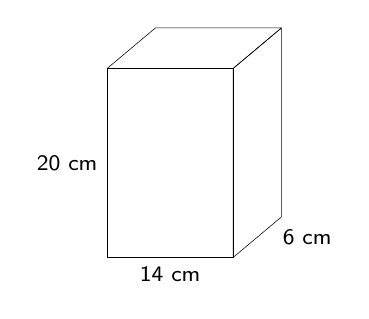
\begin{tikzpicture}[scale=0.8]
    \tkzDefPoints{0/0/A, 2/0/B, 2/3/C, 0/3/D}
    \tkzDrawPolygon(A,B,C,D)
    \tkzDefShiftPoint[C](40:1){E}
    \tkzDefShiftPoint[D](40:1){F}
    \tkzDrawPolygon(D,F,E,C)
    \tkzDefShiftPoint[B](40:1){G}
    \tkzDrawPolygon(B,G,E,C)
    \tkzLabelSegment[left](A,D){20 cm}
    \tkzLabelSegment[below](A,B){14 cm}
    \tkzLabelSegment[right, xshift=0.2cm](B,G){6 cm}
    \end{tikzpicture}
\end{minipage}
\begin{minipage}{0.4\textwidth}
    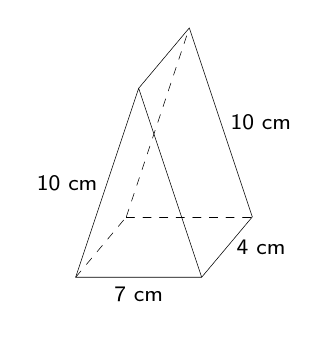
\begin{tikzpicture}[scale=0.8]
    \tkzDefPoints{0/0/A, 2/0/B, 1/3/C}
    \tkzDrawPolygon(A,B,C)
    \tkzDefShiftPoint[A](50:1.25){D}
    \tkzDefShiftPoint[B](50:1.25){E}
    \tkzDefShiftPoint[C](50:1.25){F}
    \tkzDrawSegments(B,E C,F E,F)
    \tkzDrawSegments[dashed](A,D D,E D,F)
    \tkzLabelSegment[right](B,E){4 cm}
    \tkzLabelSegment[right](E,F){10 cm}
    \tkzLabelSegment[left](A,C){10 cm}
    \tkzLabelSegment[below](A,B){7 cm}
    \end{tikzpicture}
\end{minipage}
\end{example}

\newpage 

\begin{tcolorbox}[colframe=black!20!white, opacitybacktitle=0.1, coltitle=black, title=\textbf{Isometric Drawing}]
A drawing that shows a corner view of a 3-D figure.

\begin{itemize}
    \item Shows the top, front, and side of a figure.
    \item Isometric dot paper can be used to assist in the drawing.
\end{itemize}
\end{tcolorbox}
\smallskip 

\begin{example}
Draw each figure as an isometric drawing.
\begin{multicols}{2}
    \begin{enumerate}[(a)]
        \item \mbox{} \newline 
        \item \mbox{} \newline 
    \end{enumerate}
\end{multicols}
\begin{minipage}{0.5\textwidth}
    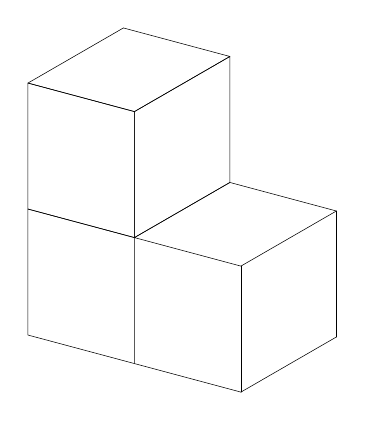
\begin{tikzpicture}[scale=0.8]
    \tkzDefPoints{0/0/A, 0/2/B, 0/4/C}
    \tkzDefShiftPoint[A](-15:1.75){D}
    \tkzDefShiftPoint[B](-15:1.75){E}
    \tkzDrawPolygon(A,D,E,B)
    \tkzDefShiftPoint[C](-15:1.75){F}
    \tkzDrawPolygon(B,C,F,E)
    \tkzDefShiftPoint[C](30:1.75){G}
    \tkzDefShiftPoint[F](30:1.75){H}
    \tkzDefShiftPoint[E](30:1.75){I}
    \tkzDefShiftPoint[D](30:1.75){J}
    \tkzDrawPolygon(C,F,H,G)
    \tkzDrawPolygon(E,F,H,I)
    \tkzDefShiftPoint[D](-15:1.75){K}
    \tkzDefShiftPoint[J](-15:1.75){L}
    \tkzDefShiftPoint[I](-15:1.75){M}
    \tkzDefShiftPoint[E](-15:1.75){N}
    \tkzDrawPolygon(E,I,M,N)
    \tkzDrawSegments(L,M N,K D,K L,K)
    \end{tikzpicture}
\end{minipage}
\begin{minipage}{0.4\textwidth}
    \raisebox{0.5in}
    {
    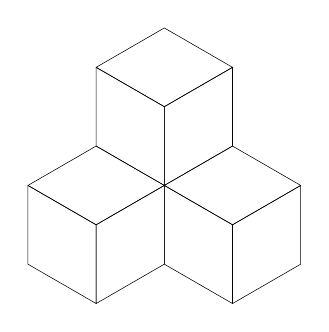
\begin{tikzpicture}
    \tkzDefPoints{0/0/O, 0/1/A, 0/-1/K}
    \tkzDefShiftPoint[A](30:1){F}
    \tkzDefShiftPoint[A](150:1){D}
    \tkzDefShiftPoint[D](30:1){E}
    \tkzDefShiftPoint[O](30:1){G}
    \tkzDefShiftPoint[O](150:1){P}
    \tkzDefShiftPoint[O](-30:1){C}
    \tkzDefShiftPoint[G](-30:1){H}
    \tkzDefShiftPoint[K](-30:1){J}
    \tkzDefShiftPoint[J](30:1){I}
    \tkzDefShiftPoint[O](210:1){B}
    \tkzDefShiftPoint[K](210:1){L}
    \tkzDefShiftPoint[B](150:1){N}
    \tkzDefShiftPoint[L](150:1){M}
    \tkzDrawPolygon(A,D,E,F)
    \tkzDrawPolygon(O,A,F,G)
    \tkzDrawPolygon(O,A,D,P)
    \tkzDrawPolygon(O,G,H,C)
    \tkzDrawPolygon(O,C,J,K)
    \tkzDrawPolygon(C,H,I,J)
    \tkzDrawPolygon(O,B,L,K)
    \tkzDrawPolygon(O,P,N,B)
    \tkzDrawPolygon(B,N,M,L)
    \end{tikzpicture}
    }
\end{minipage}
\end{example}

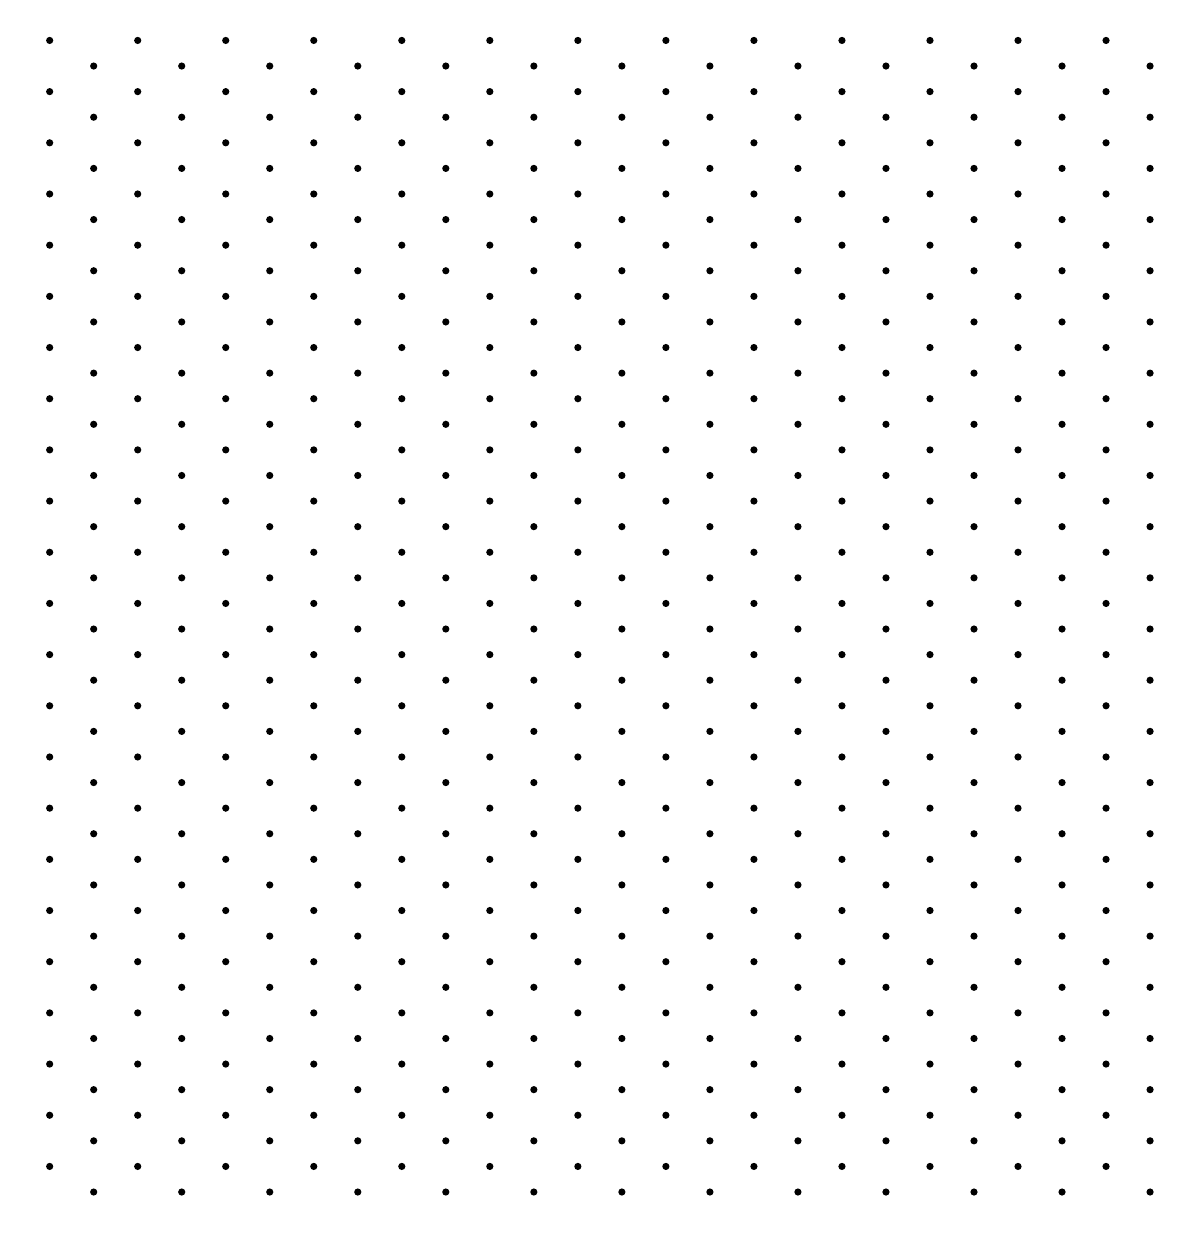
\begin{tikzpicture}[x={(0.86cm,0.5cm)},y={(-0.86cm,0.5cm)}, scale=0.65]
\clip (6,16.5) rectangle (42,26.5);
\foreach \x in {0,...,42}
    \foreach \y in {0,...,42}
    {
    \fill (\x,\y) circle (2pt);
    }
\end{tikzpicture}

\end{document}
